\begin{frame}
\frametitle{Peripheral Component Interconnect}
\framesubtitle{Motivation}
\begin{itemize}
  \item<1-> PCI впервые была предложена в 1992 компанией Intel
    \begin{itemize}
      \item в это время получили распространение ОС с GUI (Windows 3.1, OS/2);
      \item GUI требует высокой пропускной способности;
      \item другая задача - предоставить универсальный стандарт для подключения
            устройств;
      \item PCI устройства имеют более или менее одинаковый интерфейс;
    \end{itemize}
  \item<2-> Шины использовавшиеся до PCI:
    \begin{itemize}
      \item ISA - 16 MB/s;
      \item EISA - 32 MB/s;
      \item VLB - 127 MB/s;
    \end{itemize}
\end{itemize}
\end{frame}

\begin{frame}
\frametitle{Peripheral Component Interconnect}
\framesubtitle{Overview}
\begin{figure}
  \centering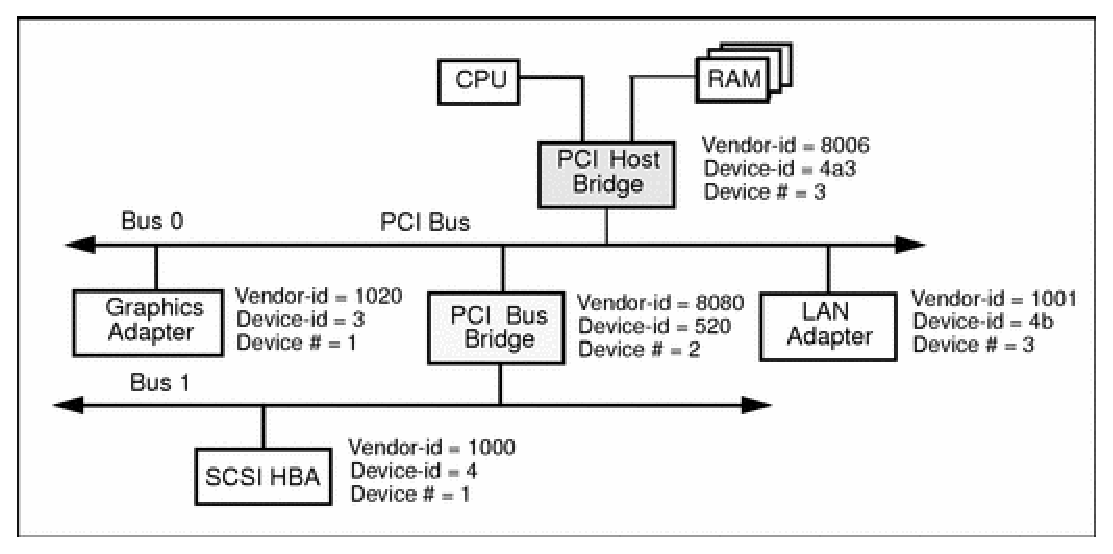
\includegraphics[width=.8\linewidth]{pci}
  \caption{PCI Local Bus Overview}
\end{figure}
\end{frame}

\begin{frame}
\frametitle{Peripheral Component Interconnect}
\framesubtitle{PCI Protocol}
\begin{itemize}
  \item Все устройства соединеные через PCI пользуются одним протоколом:
    \begin{itemize}
      \item каждая передача состоит из двух или более фаз: адресаная фаза и,
            собственно, одна или более передача данных (впрочем нас это не
            сильно волнует);
      \item в каждой передаче участвуют два устройства: Master и Target;
      \item данные передаются, если оба устройства подтвердили готовность;
    \end{itemize}
\end{itemize}
\end{frame}

\begin{frame}
\frametitle{Peripheral Component Interconnect}
\framesubtitle{Addressing}
\begin{itemize}
  \item PCI определеяет три различных адресных пространства:
    \begin{itemize}
      \item пространство памяти (Memory Address Space) - отображается физическую
            память;
      \item пространство ввода/вывода (I/O Address Space) - отображается на
            порты ввода/вывода (команды in/out в x86);
      \item конфигурационное пространство (Configuration Address Space) - может
            отображаться как на память, так и на I/O Space, но обычно используют
            память;
    \end{itemize}
\end{itemize}
\end{frame}

\begin{frame}
\frametitle{Peripheral Component Interconnect}
\framesubtitle{Configuration Space}
\begin{itemize}
  \item Каждое (почти) устройство должно поддерживать Configuration Address
        Space:
    \begin{itemize}
      \item каждое устройство предоставляет некоторое пространство из 256 байт;
      \item это пространство имеет фиксированный заголовок;
      \item через Address Space возможно идентифицировать, отслеживать состояние
            и даже конфигурировать устройство
    \end{itemize}
\end{itemize}
\end{frame}

\begin{frame}
\frametitle{Peripheral Component Interconnect}
\framesubtitle{Configuration Space}
\begin{figure}
  \centering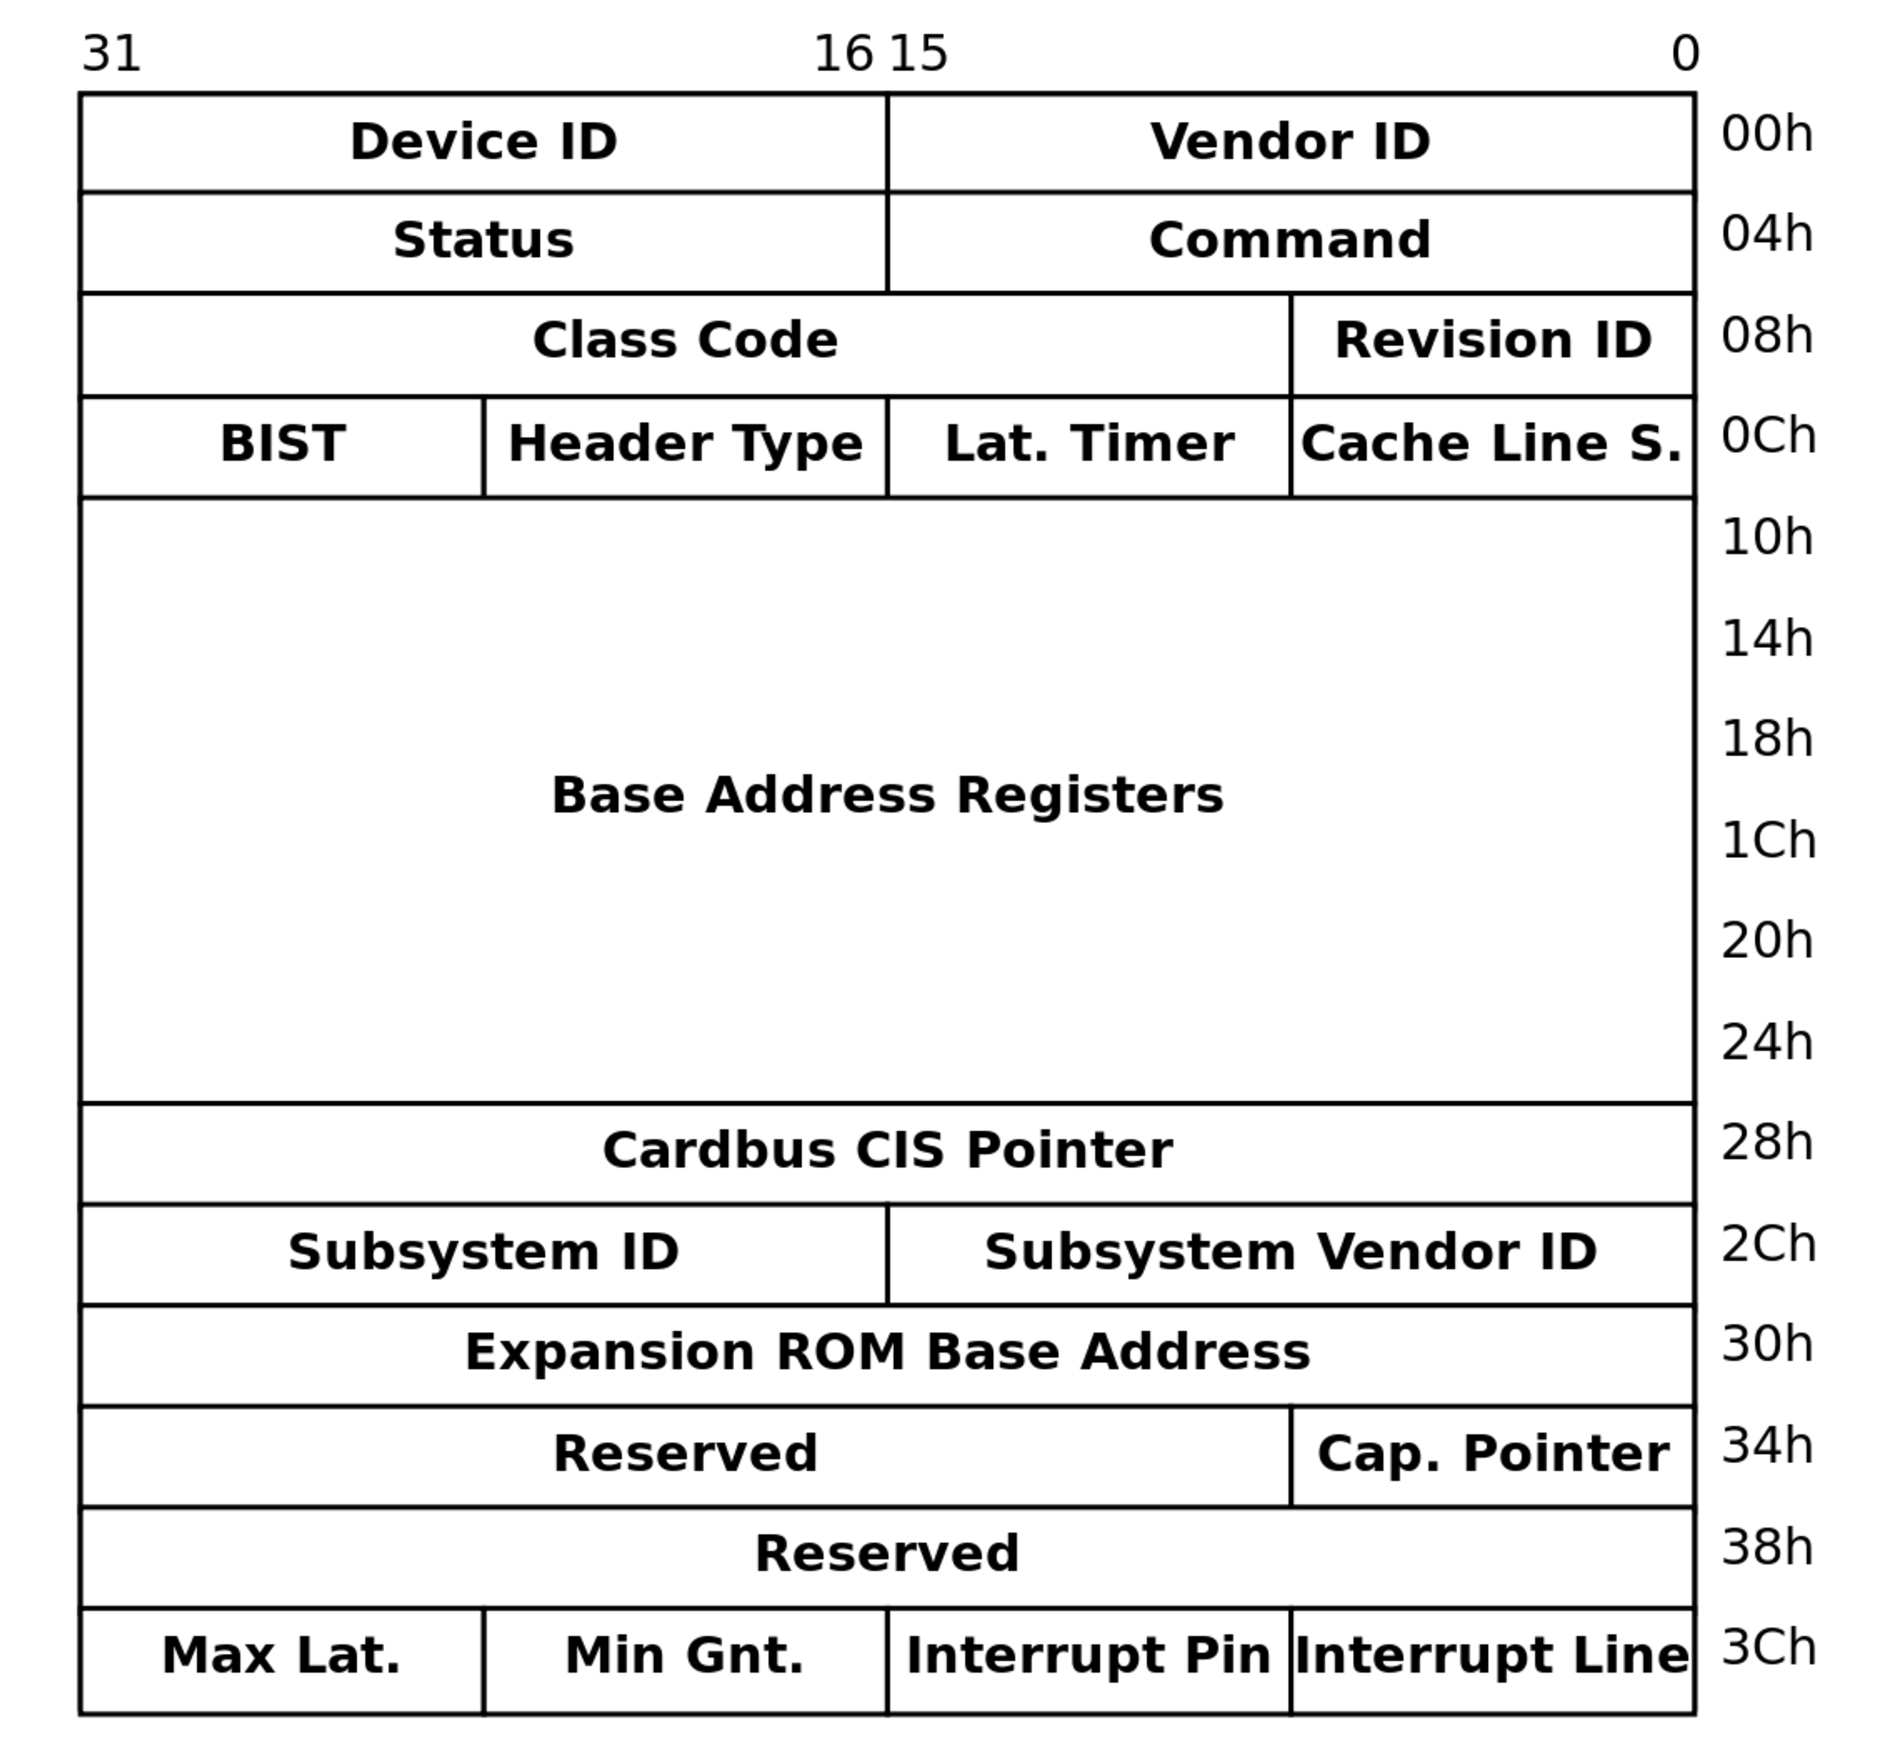
\includegraphics[width=.6\linewidth]{pci-config}
  \caption{PCI Device Structure}
\end{figure}
\end{frame}

\begin{frame}
\frametitle{Peripheral Component Interconnect}
\framesubtitle{Device Identification}
\begin{itemize}
  \item Vendor ID - идентифицирует производителя, назначеяется специальной
        организацией (PCI SIG);
  \item Device ID и Revision ID - иденифицируют конкретное устройство,
        определяются производителем;
  \item вы можете получить эту информацию не зная ничего об устройстве и даже не
        имея драйвера устройства:
    \begin{itemize}
      \item зная эту информацию вы можете автоматически найти и загрузить нужный
            драйвер;
    \end{itemize}
\end{itemize}
\end{frame}

\begin{frame}
\frametitle{Peripheral Component Interconnect}
\framesubtitle{Device Control}
\begin{figure}
  \centering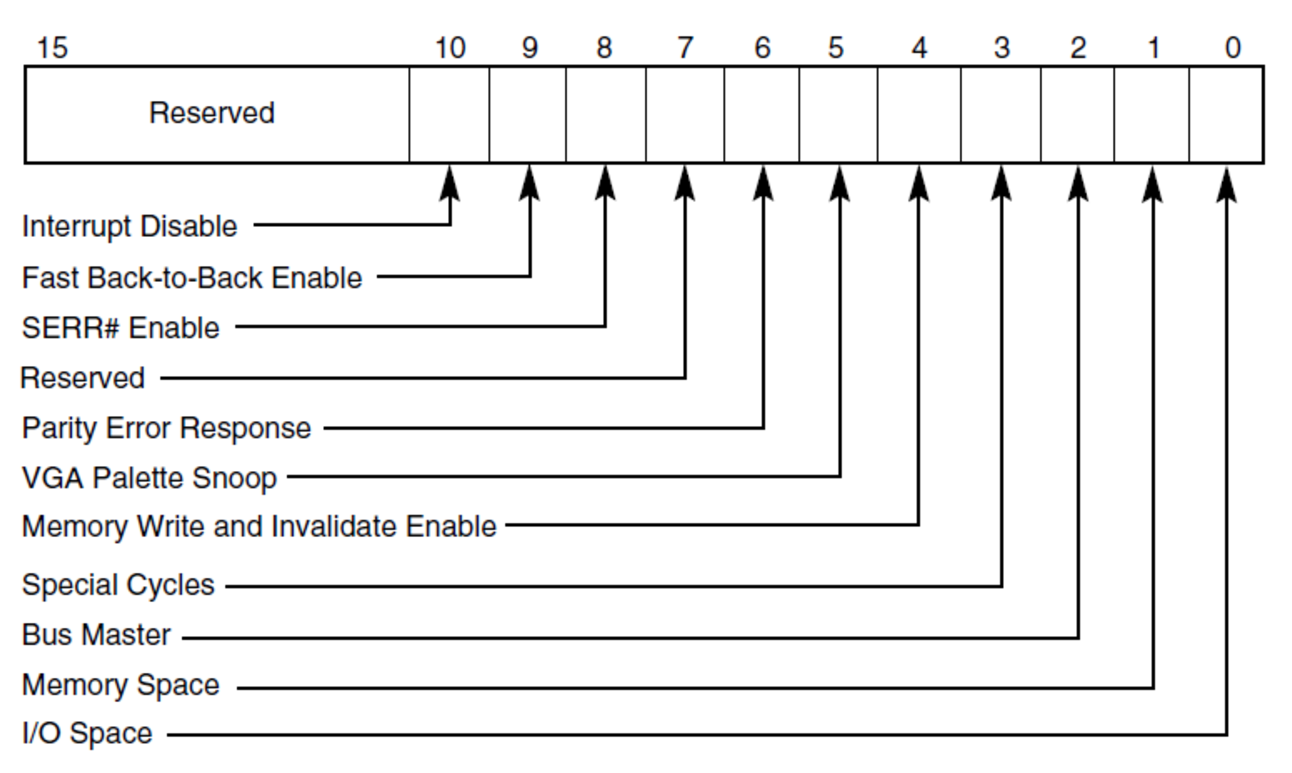
\includegraphics[width=.5\linewidth]{pci-command-reg}
  \caption{PCI Command Register Layout}
\end{figure}
\begin{itemize}
  \item Command Register осуществялет базовое управление:
    \begin{itemize}
      \item запишите 0 и устройство будет игнорировать обращения вне
            Configuration Address Space;
      \item отдельные биты могут поддерживаться или нет;
    \end{itemize}
\end{itemize}
\end{frame}

\begin{frame}
\frametitle{Peripheral Component Interconnect}
\framesubtitle{Device Configuration}
\begin{itemize}
  \item<1-> Главная особенность PCI заключается в конфигурируемости:
    \begin{itemize}
      \item теперь устройство больше не привязано к конкретным адресам в памяти,            в пространстве ввода/вывода или прерываниям;
      \item эта информация доступна ОС в унифичрованном виде через Configuration
            Address Space;
    \end{itemize}
  \item<2-> Например:
    \begin{itemize}
      \item Interrupt Line говорит какой номер прерывания использует устройство;
      \item Base Address Registers позволяют указать/узнать на какие адреса в
            памяти или в I/O Space отображены регистры и буферы устройства;
    \end{itemize}
\end{itemize}
\end{frame}

\begin{frame}
\frametitle{Peripheral Component Interconnect}
\framesubtitle{Base Addresses}
\begin{itemize}
  \item<1-> Устройство:
    \begin{itemize}
      \item устройству могут быть нужны какие-то участки памяти или I/O Space
            для работы или общения с драйвером;
      \item оно описывает размер и тип этих участков в Base Address Registers;
    \end{itemize}
  \item<2-> BIOS (или другое ПО запускаемое при старте системы):
    \begin{itemize}
      \item определяет количество памяти в системе;
      \item перечисляет устройства в системе и выделяет им память и записывает
            адрес в специальном формате в Base Address Registers;
      \item создает карту памяти и передает ее ОС;
    \end{itemize}
\end{itemize}
\end{frame}

\begin{frame}
\frametitle{Peripheral Component Interconnect}
\framesubtitle{Interrupt Sharing}
\begin{itemize}
  \item PCI шина может использовать до 4 различных прерываний (забывая про MSI):
    \begin{itemize}
      \item естественно, вы не можете выделить по прерыванию на устройство;
      \item естественно, какие-то устройства будут использовать одно прерывание;
      \item PCI устройства должны предоставить возможность проверить,
            сгенерировало ли оно прерывание или нет;
      \item но стандарт PCI не определяет каким образом - драйвер устройства
            должен это знать;
    \end{itemize}
\end{itemize}
\end{frame}

\begin{frame}
\frametitle{Peripheral Component Interconnect}
\framesubtitle{Configuration Space Access}
\begin{itemize}
  \item<1-> Configuration Address Space содержит структуры не зависимые от железа:
    \begin{itemize}
      \item это хорошо для драйверов - PCI драйвер в хорошо спроектированной ОС
            не требует портирования на разные архитектуры;
    \end{itemize}
  \item<2-> Способ доступа к Configuration Address Space зависит от архитектуры
    \begin{itemize}
      \item а еще от версии PCI (их уже довольно не мало);
      \item хорошо спроектирвоанная ОС скрывает эти детали;
    \end{itemize}
\end{itemize}
\end{frame}

\begin{frame}
\frametitle{Peripheral Component Interconnect}
\framesubtitle{Configuration Space Access}
\begin{itemize}
  \item Адрес в Configuration Address Space состоит из:
    \begin{itemize}
      \item номера шины - в системе может быть несколько шин PCI;
      \item номера слота на шине - к одной шине может быть подключено несколько
            устройств;
      \item функции - специфичное для PCI понятие, PCI устройство может
            предоставлять несколько "функций";
      \item смещение внутри PCI Device Structure;
    \end{itemize}
\end{itemize}
\end{frame}

\begin{frame}
\frametitle{Peripheral Component Interconnect}
\framesubtitle{Configuration Space Access}
\begin{itemize}
  \item<1-> Conventional PCI (или просто PCI) в IBM PC использует I/O порты:
    \begin{itemize}
      \item для задания адреса 32 битный порт с адресом 0xCF8;
      \item для чтения/записи данных 32 битный с адресом 0xCFC; 
    \end{itemize}
  \item<2-> PCI Express отображает Configuration Address Space в память
    \begin{itemize}
      \item найти базовый адрес можно в одной из таблиц ACPI (MCFG);
    \end{itemize}
\end{itemize}
\end{frame}

\begin{frame}
\frametitle{Peripheral Component Interconnect}
\framesubtitle{Enumeration}
\begin{itemize}
  \item После того как мы получили доступ к Configuration Address Space мы можем
        легко перечислить все PCI устройства в системе:
    \begin{itemize}
      \item перебираем номера шин от 0 до 255 и номера устройств от 0 до 31;
      \item проверяем есть ли такое устройство в системе;
      \item для проверки просто запрашиваем Vendor ID, если не 0xffff, значит
            устройство присутствует;
    \end{itemize}
\end{itemize}
\end{frame}
